\chapter{Inferring Interestingness of Tweets based on Information Flow Through the Network}


Mention:
\begin{itemize}
\item How this chapter builds upon network stuff in previous chapter
\item We hope to compare and contrast two better ways of predicting retweet volume \emph{and} interestness
\item What needs to be improved (speed, usability - more users with more followers etc.)
\item Why do improvements need to be made?
\item How is this useful, and how does first chapter relate to work done here?
\end{itemize}

Discuss:
\begin{itemize}
\item Does not use network to simulate tweets - instead uses a set of user features
\item Previous chapter shown how basic features can be used to generate a scale-free network, which is what twitter is
\item Use these features as input attributes of a new machine learning technique model.
\item This method does not use a network or model individual user decisions
\item Trained on a set of that particular user's tweets with the retweet outcome of integer type
\item A new tweet modelled with the regression outputs a retweet volume prediction without having to simulate the Tweet's travels through the network. 
\item Discuss about the machine learning approach used (logistic regression and how it works)
\item Talk about the 'binning' of retweet outcome volumes and its approaches (distribution dependent / independent, tables of precisions, etc.)
\item Link 'retweet volume' to 'retweet group size'
\end{itemize}

Research in the previous chapter focussed on researching the effect of the social graph on retweet propagation characteristics. From this, a methodology, displaying a range of various shortcomings, emerged based on the models and simulations utilised in the graph analyses. In this chapter, the methodology is modified with the aim of improving its performance and increasing the range of use-cases it is appropriate for. Since the social structure was found to play an important role in propagation, many network and user features are taken into account throughout the improvements.\\
In addition, modifications are made in order to provide an indication of \textit{how} interesting a piece of information is estimated to be, and more about this particular component is discussed in later sections.

The proposed methodologies also relate to the differences highlighted between a Tweet's raw popularity, as indicated by its retweet count, and hos interesting the Tweet actually is to those who read it. It has been shown that making retweet predictions against models trained with a large number of features can be accurate \cite{zhu11}, but in this work, the focus is more on the Tweet's content and beyond the static features.\\
That is, that when comparing Tweet popularity, then there may be some content, either within the Tweet itself or perhaps in a resource indicated by a URL contained in the Tweet, that makes the Tweet stand out to its recipients and to cause the aforementioned notion of \textit{affective stimulation} \cite{xu07} to its viewers.

Of course, this brings about the notion of information \textit{relevance}, and the fact that the same Tweet could be very boring or irrelevant to one user, and very interesting to another. In this work we focus on \textit{global} (or `average') interest, where interestingness inferences are made for the general case. It is considered that Tweets that are retweeted more than expected within their authors' local networks, relative to the usual retweet count of the authors' other Tweets, are also likely to be of interest to a wider audience, especially since they are now more likely to penetrate through the social graph enough to be received by users in different communities..
 
As such, the focus of the work in this chapter is that of adapting the inference methodology in order to develop a technique for accurately \textit{quantifying} the interestingness of tweets. This is concerning universal relevance in terms of highlighting interesting Tweets from the noise. In particular, there are two main improvements of the previous methodology to be made;
\begin{itemize}
    \item Improve method for generating the \textit{expected} retweet count of a Tweet (in terms of accuracy and range of application)
    \item Expand the binary retweet interesting inference into a more useful scale in order to support \textit{ranking} of interesting information.
\end{itemize}


\section{User Influence}
As has previously been posited, of importance to this work is the difference between the retweet count of a Tweet and the interestingness of the Tweet. An example in the Background chapter was provided, which related to the case of Justin Bieber. His account, \texttt{@justinbieber}, is one of the most influential on Twitter, with nearly 50 million followers at the time of writing. His Tweets receive an average of around 50-120 thousand retweets per Tweets, and they rarely receive fewer than 40,000 retweets.\\
Since an average Twitter user would generally attract a maximum of a few hundred followers, and would normally receive very few, if any, retweets per Tweet. A particularly interesting Tweet from such a user may be retweeted, for example, between 5-20 times. It is therefore apparent that, in the general case, an uninteresting Tweet from an influential user may receive 50,000 retweets, and an exceptionally interesting Tweet from a less-influential user may be retweeted 30 times. It is therefore clear that user influence dictates that this value cannot alone be indicative of Tweet interest.

However, since interestingness \textit{does} have an effect on an a user's individual retweet decision, this absolute retweet count can be used as part of the method for generating an interestingness \textit{score} for a Tweet.


\section{Interestingness Scores}
To address the notion of interest quantification, a scoring scheme is hereby introduced, allowing certain interesting Tweets to be ranked as `more interesting' than other interesting Tweets. This, in itself, is an improvement over the previous method, which allowed only for Tweets to be labelled as `interesting' or `non-interesting'.

Similar to the previous method's \textit{comparison} between the observed and expected retweet counts, the new scoring technique is based now on the \textit{difference} between the two counts. The general idea and potential use-case for this is that if a score is known for a set of Tweets, then these can be used as a basis for ordering information as part of information retrieval or an information delivery system, where Tweets can be displayed to users in a more useful way and where interesting Tweets could be brought forward to users who don't follow the source user or a retweeter, and thus deliver information to an interested user, yet without him or her having to know about it first.

Essentially, the notion scoring stems from the following scenario. Consider two Tweets, $A$ and $B$, which have the following properties;
\begin{itemize}
    \item $\ec{A} = 3000$ and $\rc{A} = 3010$
    \item $\ec{B} = 5$ and $\rc{B} = 15$
\end{itemize}
Where $\ec{A}$ represents the expected retweet count of $A$.

In this case, both Tweets would have been flagged as `interesting' under the previous scheme (although, in reality, the method would not be able to model users who are typically expected to achieve 3,000 retweets). However, it is clear that, despite the \textit{difference} between the counts being equal, Tweet $B$'s observed retweet count is actually much more significantly proportionately greater than what was expected, and is therefore likely to be more significantly interesting.

Since the proportionate difference is the key to this, the interestingness score, $\score{t}$, for Tweet $t$ is hereby simply given by;
\[
\begin{array}{cc}
 \score{t} = \frac{\ec{t}}{\rc{t}}
\end{array}
\]

This provides a positive score where;

\[
\score{t}
	\begin{cases}
		> 1		&	\text{indicates } t	\text{ is interesting} \\
		\leq 1	&	\text{indicates } t	\text{ is non-interesting}
  \end{cases}
\]

And where $\score{A} > \score{B}$ implies that $A$ is more interesting than $B$.

Since this methodology relies on data collection from Twitter in order to obtain the observed retweet counts, it involves extracting a snapshot of the state of the evaluated Tweets at one stage during their lifetime. Since Tweets are not removed over time, unless they are deleted by their author, they can be discovered and retweeted at any time after their composition and posting.\\
The work in this chapter assumes that the most significant portion of retweet activity for a specific Tweet has already occurred by the time the information on the Tweet has been collected. Indeed, the authors of \cite{kwak10} carried out investigative analyses into various temporal retweet brhaviours, and discovered that, on average, that a Tweet receives around 75\% of its retweets within the first day of being posted. 50\% of the retweets of a Tweet take place within the first \textit{hour} of the Tweet being posted.\\
Due to this, and to ensure that the retweet count collected is mostly representative of the Tweet's exraploated `final' retweet count, only Tweets that had been posted at least one day ago were considered for experimentation.


\section{Further Adaptations of the Inference Methodology}
In the previous chapter, it was noted how it was necessary to improve the method used for producing a Tweet, $t$'s, expected retweet count, $\ec{t}$. Problems with the previous method dictated that the method could only work under certain restrictions. In particular, that the user must have a small enough local network (in practice, a follower count of more than 500 or so made the method very unsuitable), and that, due to this, Tweets only attracting very few retweets could effectively be simulated. In addition, the interestingness inferences made were not significantly accurate, although this is likely due to a combination of the aforementioned issue providing much less room for error and the fact that the interestingness decision was only binary.

A new method is hereby proposed for carrying out the prediction for the value of $\ec{t}$. This method is immediately more superior to the previous, as only a very small amount of data (if any) is required to be collected from Twitter. This means that inferences on Tweet interestingness could be made on demand\footnote{Not `live' due to retweet action relies on time to occur.}.\\
Essentially, the method involves creating a classifier model capable of producing a base-line expected retweet count for a given Tweet and its relationship with its author. In this case, the classifier would be trained with the Tweet's actual retweet \textit{count} instead of the binary retweet decision used previously, and it would not require the simulations of the user's local network. Many more features regarding the Tweet, and its conetent, and its author are used to represent the particular user-Tweet information required for generating the predictions.

Since the graph structure clearly has an impact on message propagation, then it was felt that a significant consideration should be made towards including features relating to the interconnection of users, such as follower counts, Tweet rate, and information on a sample of friends and followers. More detail on the features used is provided in later sections.

In general, the newly proposed methodology follows these basic steps:
\begin{enumerate}
    \item Collect sufficent data from Twitter to train a classifier with an appropriate set of features. The trained model is known as the `global' model;
    \item Obtain a Tweet, $t$, and extract its own features as well as information about its author and its author's network properties;
    \item Classify the Tweet's features against the trained classifier to produce a retweet count prediction, $\ec{t}$ for this feature instance;
    \item Calculate \score{t} through using this $\ec{t}$ value and the known $\rc{t}$.
\end{itemize}

In addition to this `global' model, a `user' model was proposed to be built for each user being evaluated. This user model would be much smaller, as it would only contain information on that user's historical Tweets, but would be capable of providing a second value for $\ec{t}$. With two such values, two scores could be generated by comparing the static $\rc{t}$ to each in turn.

As such, the two scoring mechanisms work as follows;
\[
    \gscore{t} = \frac{\rc{t}}{\ec{t}_1}
\]
\[
    \uscore{t} = \frac{\rc{t}}{\ec{t}_2}
\]


\section{Retweet Volumes as Nominal Attributes}
Most machine learning classifiers are not useful in accurately predicting the outcome of a feature of a large-ranging and continuous data type. Instead, the performance can be greatly improved when predicting from a limited range of discrete ranges, or `nominal' data.

Thus, in order to help improve the accuracy of $\ec{t}$ predictions, it was decided to convert the retweet count feature into a nominal data type for the purposes of training the model and making classifications. By `binning' the retweet counts into categories representing interval ranges, there would be fewer outcome possibilities, and thus the \textit{confidence} of classifcation could be greater.

The values for $\score{t}$ would then be determined through the ratio of $\rc{t}$ to the upper-bound of the nominal range category containing $\ec{t}$.


\subsection{Binning the Retweet Counts}
Since a trained classifier is only generally able to make predictions on features and values it has prior knowledge of, the bin ranges for each category must be equal in both the training feature data and the testing feature data. If the available nominal values for an instance feature representing a Tweet has a different set of category ranges to that in the trained classifier model, then it is likely that a prediction cannot be generated for this instance. It was therefore necessary to consider this when determining a method for binning the retweet counts.

There are various ways in which the counts could be binned, and all begin with a decision on the number of bins to use. The varying performance of this factor is considered later.

Initially, retweets were binned in a \textit{linear} fashion. That is, that the full range of retweet counts in the training set was calculated and then split into bins such that each category had an equal a range as possible. If there were no cases where $\rc{t} = 0$, then a category representing $[0,l)$, where $l$ is the minimum value for the lowest range, was pre-pended to the set of available nominal categories. Similarly, in all cases, the interval $[m+1,\infty)$ was appended to the set of categories, where $m$ is the maximum value in the highest range. This dictates that no Tweet in the training set can have a value for $\rc{t}$ in this category, and thus this allows any Tweet to potentially have $\score{t} > 1$. For example, if a training set of Tweets had a total range of values for $\rc{t}$ being between 1 and 20 was binned into four ranges, then the following interval categories would be applicable:
\[
    [0,1) [1,6) [6,11) [11,16) [16,21) [21,\infty)
\]

Since the distribution of retweet counts (expressed through retweet group sizes) is known \cite{webberley11}, then it is clear that this binning methodology would produce bins containing a very non-uniform distribution of Tweets, where the lower bin ranges would contain many Tweets and the cardinality of each category would decrease exponentially as the ranges become higher. This means that there would be fewer feature instances representing Tweets with larger retweet counts.\\
 Indeed, when training classifiers and running cross-validations on these, this binning scheme demonstrated a high accuracy of predictions on Tweets with lower values for $\rc{t}$ and a low accuracy for Tweets with higher counts. It would be more appropriate, and better address the desire for more universal use-cases expressed earlier in this and the previous chapter, if the accuracy of predictions could be more uniform across the bin ranges.

Various other methodologies were implemented, which eventually evolved into a histogram-based responsive  binning algorithm. Essentially, this algorithm involved is based around the initial calculation for the projected size of each bin, which is based on the total number of Tweets to be categorised and the target number of bins. Each bin was then filled according to the interval range specifying the bounds of that bin, and in such a way such that each retweet count frequency would only be present in one bin. For example, all of the retweets achieving one retweet would be placed in the single bin encompassing this value.\\
As such, after the intervals representing the bin bounds have been produced, then these represent the nominal categories for the retweet count feature in each instance for training and testing against the classifier.



\newfloat{algorithm}{H}{lop}
\begin{algorithm}
\caption{Algorithm for producing intervals for bin categories for $\rc{t}$ values.}
\begin{algorithmic}[1]
\Procedure{generate\_intervals}{set of Tweets $T$, number of bins $B$}
    \State $C\gets$ empty list \Comment{To hold ordered retweet counts}
    \State $I\gets$ empty list \Comment{To hold bin range intervals}
    \ForAll{$t \in T$}
        \State Add $\rc{t}$ to $C$
    \EndFor
    \State Sort $C$ into ascending order 
    \State $M\gets\max(C)$ \Comment{Highest instance of $\rc{t}$}
    \State $T\textrm{Sum}\gets\frac{|C|}{B}$ \Comment{Number of Tweets in each bin}
    \State $H\gets$ empty dictionary \Comment{Histogram of retweet count distribution}
    \Statex
    \ForAll{$c \in C$}
        \If{$c \in H$}
            \State Increment $H_c$
        \Else
            \State $H_c\gets0$
        \EndIf
    \EndFor
    \ForAll{$i$ in range $M+1$}
        \If{$i \in H$}
            \State $s = s + H_i$
        \EndIf
        \If{$s \geq T\textrm{Sum}$}
            \State Add $i$ to $I$
        \EndIf
    \EndFor
    \State Return $I$
\EndProcedure
\end{algorithmic}
\label{algo2}
\end{algorithm}
 
This new responsive method more readily supports more uniform bin sizes, and copes with this by expressing exponentially larger bin \textit{ranges}. As such, the distribution of bin sizes is generally described by a distribution simular to that shown in Figure \ref{fig:bin-hist}. As with the linear method, the interval $[0,l)$ is pre-pended, where necessary, and $[m+1,\infty)$ is always appended in addition to the intervals produced by the algorithm.

\begin{figure}[h]
\centering
\begin{tikzpicture}
\begin{semilogyaxis}[
    symbolic x coords={[0-1), [1-2), [2-3), [3-4), [4-5), [5-100)},
        ylabel=Cardinality of bin,
		xlabel=Bins,
        ybar,
        bar width=7pt,
        yticklabels={,,},
        xticklabels={,,}
        ]
   \addplot[plot 0,bar group size={0}{1}]
        coordinates {([0-1),100) ([1-2),50)  ([2-3),50) ([3-4), 50) ([4-5), 50) ([5-100), 25)};
        
\end{semilogyaxis}
\end{tikzpicture}
\caption{Example distribution of retweet count bin cardinalities under the responsive binning algorithm}
\label{fig:bin-hist}
\end{figure}

This method is responsive in that the bin ranges adapt to the variety and number of retweet counts available, and always attempts to produce a similar number of bins to what is requested. However, due to the disproportinately large number of small retweet groups, the bin sizes cannot be entirely uniform and means that the number of intervals returned will be smaller than the number requested.\\
This also stems from the fact that a single retweet count cannot exist in more than one bin concurrently; for example, if the interval $[0,2)$ existed in a scenario, and the number of Tweets with retweet count equal to 0 or 1 is greater than the value for $T\textrm{Sum}$, which is often the case, then this will result in a larger bin. Without this particular feature, a Tweet may be categorised into more than one bin, causing the prediction accuracy to be reduced. 

Due to this dynamicity, the bin ranges and cardinalities produced by the algorithm vary across different datasets. As a result, the nominal bin categories generated for producing the value for $\uscore{t}$ from the user model trained from the complete set of collected Tweets posted by $\aut{t}{O}$ would be different from those categories generated for a different user. The intervals in each bin category are therefore reflective of the various different number of retweets that each author's Tweets are likely to receive. 


\section{`Twitter is a Memepool'}
In 1976, Richard Dawkins coined the term `meme' to be defined as a ``unit of cultural transmission'' \cite{dawkins76}. The general idea behind memetics is as an analogy to biological genetics except, unlike genes, memes are entirely non-physical and represent a cultural idea or aspect or another human-based behaviour. The rise of social networks on the Internet has allowed the spread of memes to grow to the extent that they are sometimes now even \textit{represented} by physical constructs, such as images.

In genetics, a gene is a physical entity containing information and instructions. It is a unit of genetic inheritance, in that they are passed from parent to offspring through the act of reproduction, and the result of an organism having a gene will express the features represented by that particular gene. These genes contain instructions that make up the features of an individual, such as physical characteristics like eye colour and height, and non-physical characteristics, including various aspects of personality.\\
Organisms exist in an evironment that also has features, such as humidity, altitude, temperature, relations to other organisms, and so on. If the genes of an organism are such that they cause the individual to be well-suited to its environment, then that organism has a better chance of survival and, therefore, a better chance of achieving reproduction.

Memes are similar in that they are effectively made up of a set of features, or `memome', such as the wordings of a particular phrase, or their relevance to other cultural aspects. These enable the meme to be less or more likely to be replicated in different environments, which is made up of the humans exposed to it and the interactions between them. For example, an Internet meme relating to the Star Wars movies would likely have a greater chance of being reproduction, through discussion and reposting, in an environment comprising a set of science-fiction fans than when amongst more mixed-interest groups.

The meme is also a useful analogy in this thesis when describing the way in which Tweets undergo replication within Twitter. Like a meme, a Tweet has a specific set of features, such as the text it contains, the inclusion of any mentions or a URL, and so on, and it exists within an environment consisting of a set of interconnected users on the Twitter social graph.\\
A particular Tweet would generally have a greater chance of `surviving' and being replicated, through the act of retweeting, amongst certain users intereconnected in a particular way than in other environments.

As such, the Tweet features are analogous to the \textit{genes} of a genome, and the arrangement and type of users on the social graph that receive the Tweet and have an opportunity to assist in its propagation comprise the Tweet's \textit{environment}. Since the environment has previously been found to have a large effect on propagation, then these features are useful aspects to include as part of the improved methodology covered in this chapter.


\section{Generating Values for $\ec{t}$}
In order to generate the estimated retweet counts, a trained machine learning classifier is needed to make predictions on a set of feature instances. This section covers an overview of the classifier used for this purpose including a justification in terms of an analysis of its performance.


\subsection{Machine Learning Classifier}
An overview of machine learning classifiers and their processes was provided in the previous chapter. In that case, a logistic regression was used to generate a prediction on a binary retweet decision based on a small number of features. If the retweet count for the Tweet being trained or tested was greater than zero, then the retweet decision would be positive (\textsc{True}). Otherwise, the decision was negative (\textsc{False}).

Presently, the new methodology involves the prediction of a retweet count category from a set of nominal values of greater cardinality than two. As mentioned, the instances of a particular Tweet and its evironment are categorised based on the value of the retweet count of the Tweet. Although this means that a degree of accuracy is sacrificed when training the classifier, it does mean that there are fewer categories for predictions on test Tweet feature instances, providing a higher confidence in each prediction made.

The Bayesian network machine learning classifier was elected for use for the purposes required in this chapter. Use of this classifier in the social media domain is more rare than other classifiers, such as those involving a regression or a decision tree, but was selected for the various reasons highlighted later in this section.

The Bayesian network is an unsupervised classifier since its learning algorithms do not simply determine the class of the outcome, the retweet count, from the attribute features alone \cite{friedman97}. Instead, a probabilistic graph is constructed based on the dependencies between the variables. The variable attributes form the nodes of the graph and edges between the nodes denote the dependencies (or lack thereof) between them.

Thus, in the case of this research, the various Tweet and envirnomental features, including the nominal retweet count, form the nodes in the Bayesian Network. When forming the graph through training, the dependencies and their probabilistic weightings are adjusted so that an expected value for the retweet count can then be `predicted' from the values of all the other variable attributes.


\subsection{Classification Performance}
When selecting classifiers, the Weka\footnote{http://www.cs.waikato.ac.nz/ml/weka} machine learning and data mining toolkit was used to evaluate the relative performance of various types of appropriate classifiers for the task.\\
Although the accuracy of prediction was important, it would also be useful for the classifier to be \textit{efficient} in training its model and when testing future instances against it. This is so that this method could be used to produce interestingness inferences on demand and to further improve on the methodologies used in the previous chapter.

\begin{table}[h]\footnotesize
\begin{center}
\begin{tabular}{ l | c | c | c }
	Classifier	& Precision & Accuracy (recall) &  training time (secs.) \\
	\hline
	\hline 
	Simple logistic & 52\% &  56\% & 528\\
    Logistic        & 62\% &  56\% & 18\\
    SMO             & 51\% &  55\% & 1384\\
    Na\"{i}ve Bayesian & 50\% & 44\% & 0.13\\
    Bayesian network & 62\%&  64\% & 0.54
    \hline  
\end{tabular}
\end{center}
\caption{The training performance of different machine learning classifiers}
\label{table:classifierperformance}
\end{table}

The Bayesian network was found to be accurate and time efficient when evaluating the performance of the set of classifiers. The same dataset obtained midway through the general data collection (please see the relevant section below), containing a set of over 57,000 Tweets, was used in the analyses. For each Tweet instance the same retweet count binning scheme was used, and each classifier performed the same number of cross-validations against the same dataset in order to obtain the precision and recall values.


\subsection{Varying the Cardinality of Binned Retweet Counts}

Number of bins: explain how accuracy worsens as bin number increases.
Performance with different numbers of instances




\section{Training and Testing Against the Bayesian Network Classifier}
Stuffs

\subsection{Data Collection}


This paper considers only Tweets that have been retweeted using the `button' method, which is a single-click function on the Twitter website and its applications to carry out a retweet. Twitter users also sometimes imitate a retweet by copying the text of the original Tweet and prepending it with an ``RT'' followed by the original author's screen-name, which allows them to add annotations to the Tweet if they desire.\\ 
- as v 1.1 had to be used (no public timeline), so rely on detection through Twitter's retweet:true attribute.

In March 2013, a random walk was carried out through the Twitter social graph using Twitter's REST API, originating with one of this paper's author's Twitter account. Each step of the walk involved focusing on one Twitter user, collecting information on that user, and then selecting a random follower of that user. This follower then became the focus of the next step.\\
At each step, a set of the most recent Tweets from the current user were collected. The number of Tweets returned by the Twitter API differed from user to user, based on their recent Tweet-posting frequency, though usually a few hundred Tweets were yielded. In addition to their Tweets, we also collected information on the user itself and on a sample subset (up to 100, if they exist) of its friends and followers. We used a sample instead of collecting information on \textit{all} of a user's friends and followers so that we could maximise the efficiency of our method in terms of data collection. It also meant we had a snapshot of an additional 200 users in the author's local network to give the classifier a notion of the activity of this local network both upstream and downstream from the author.\\
This gave a dataset containing around 241,000 Tweets from 370 unique Twitter users and, of those Tweets, around 90,000 were cases where the retweet volume was greater than zero. The dataset was split into two datasets: a training set (90\%) and the testing set (10\%). The original dataset was split in such a way as to allow all Tweets belonging to one particular user to exist in only one of the two smaller datasets. The training set was used to train a model, as described below, and was then discarded from the rest of the experimentation.

\subsection{Data Corpora}
As discussed in the methodology section, we are interested in producing \textit{two} predictions for each Tweet; one when compared to the global set, and another from comparisons to the rest of that user's Tweets. Therefore, a new dataset was formed for each user in the testing dataset which contained the Tweets only from that particular user. For the remainder of this section, the testing dataset is the \textit{global} corpus of Tweets, and each of the individual user datasets are known as \textit{user} corpora.\\
The Bayesian Network was chosen as our classifying algorithm to produce the predictions as it was suitable for the data types of the Tweet and user features and was also found to perform efficiently in terms of precision and recall across the outcome predictions when carrying out test cross-validations against itself. The prediction precision weighted across the outcome categories was calculated to be around 70\% in cross-validation tests on the training dataset features.

\subsection{Features}
To train the Bayesian Network model, a series of new features were harvested. Generally, each of these features fell into one of two categories; user features and tweet features.
\\
The Tweet features follow the same ideas as the features used in the previous chapter: static, generally binary features that describe the structure of the Tweet. The user (or `network')  features are related more to the \emph{network} to which the Tweet belongs.\\

Features were extracted from the Tweet and user data to train the Bayesian Networks. Each Tweet is represented by an \textit{instance} of feature sets specific to that Tweet (and its author, if appropriate). In each instance the outcome feature is the retweet volume, which is categorised using the technique discussed later.\\
Since some features are static among Tweets from the same user (for example, a user's follower count), a different feature set is used to train the user models and the global model, as described below.

\subsubsection{Features for the global corpus model}
A total of 31 features were used to train the model classifier from the global data corpus.

\begin{table}[h]\footnotesize
\begin{center}
\begin{tabular}{ c | l | c }
	 Feature category	& Feature & Feature data type \\
	 \hline
	 \hline 
	& mention & \{True, False\}\\
    & Tweet length & real (numeric)\\
    & url & \{True, False\}\\
  	& hashtag & \{True, False\}\\
  	Tweet & positive emoticon & \{True, False\}\\
  	(`genome')& negative emoticon & \{True, False\}\\
  	& exclamation mark & \{True, False\}\\
  	& question mark & \{True, False\}\\
  	& starts with `RT' & \{True, False\}\\
  	& is an @-reply & \{True, False\}\\
  \hline                        
	& follower count & real (numeric)\\
    & friend count  & real (numeric)\\
	Author & verified account & \{True, False\}\\
	& status count & real (numeric)\\
	& listed count & real (numeric)\\
  \hline
  	&  max. follower count & real (numeric)\\
	&  min. follower count & real (numeric)\\
	&  avg. follower count & real (numeric)\\
    Network &  max. friend count & real (numeric)\\
	(`environment') &  min. friend count & real (numeric)\\
	&  avg. friend count & real (numeric)\\  
	&  avg. status count & real (numeric)\\  
  	& proportion verified & real (numeric)\\  
  \hline  
\end{tabular}
\end{center}
\caption{Features used to train the model from the global data corpus}
\label{table:globalfeatures}
\end{table}

The features used to train the global model are outlined in Table \ref{table:globalfeatures}. The network features apply to both the followers and friends retrieved for each author. For example, the first feature of this category, `max. follower count', represents two features referring to the maximum follower count observed in the sample of the author's followers and in the sample of the author's friends. \\
While Tweet features are permanent after the Tweet has been created, the author and network features are dynamic in that the social graph is of a constantly altering structure as links are formed and broken between users. However, in this work, we assume that the changes to these features are not significant over the Tweets collected for each user and try to minimise this by only considering recent Tweets of each user.

\subsubsection{Features for individual user models} 
The 10 Tweet features were used for training each user-based Bayesian Network to reduce redundancy in the model since the author and network features would be the same across all of the Tweets from one user.



\subsection{Testing Against the Trained Classifier}
The global and user models were then trained using the features to produce one global model and one user model for each unique author in the testing dataset, as described above.\\
To produce the global predictions, $ T_{P_G} $, each Tweet in the testing database was evaluated against the global model, which output a predicted value for the bin that Tweet is predicted to belong to.\\
The user predictions, $ T_{P_U} $ were calculated in the same way: each Tweet in the testing dataset was evaluated against the model based on the Tweet's author.\\
Each Tweet then each had two retweet volume predictions. The upper bound of the binned category assigned to each prediction was compared to the \textit{observed} retweet count to produce the two interestingness scores, $ TS_G $ and $ TS_U $, as discussed earlier.


\section{Methodology Validations}

\subsection{Planning the Result Validation}
Crowdsourcing is a technique often employed by companies and researchers to collect large amounts of data from a (often large) distribution of people or devices. Examples of this in practice include the use of surveys and user-contributed reviews (such as in Google Maps).\\
In this paper we use Amazon's Mechanical Turk service as a method for crowdsourcing interestingness validations from many people, who are known as Mechanical Turk Workers (MTWs) 

To assist in validating the interestingness scores produced for the Tweets, tests were required in which humans would be responsible for also assessing how interesting they feel the Tweets were. The predicted interesting Tweets could then be compared to the Tweets chosen as interesting through human judgement.\\
For this stage of the experimentation, certain Tweets (and users) were removed from the dataset to be tested by the humans. Since the Tweet data was collected using a random walk through Twitter, there was no governance over the content of the text in this data. Therefore, users who frequently used offensive or non-English (since the Tweets were to be validated by English-speaking individuals) language had their Tweets removed from the test set. In addition, individual `@-replies' (Tweets starting with the `@' symbol) were also stripped from the test set since these usually denote conversations on Twitter between two or more users and are unlikely to convey any interest to outsiders.


\subsection{Validating the Methodology Outcomes}
In this context, MTWs have no connection to the Tweets in the dataset, and are random users of Amazon's Mechanical Turk who decide to take the job on. Collecting the validation data in this way, and instead of using a small set of people, means that we can collect a diverse opinion on Tweet interestingness from people whom the Tweets will have varying relevance to. This helps reinforce the notion of \textit{global} interest levels, where Tweets can be interesting to a large number of users.\\
The human validations were carried out such that the MTWs were presented with questions, each of which consisting of five different Tweets from one specific author. Each question asked that the MTW select the Tweets they consider to be the most interesting of the group and that they must select at least one. MTWs were paid \$0.05 for each question they answered and there were 91 unique MTWs in total who responded to the questions.\\
The tests were under the conditions of a randomised controlled trial, such that each Tweet was assessed in three different contexts (i.e. each Tweet would appear in three different questions alongside four randomly chosen other Tweets) and that each question would be responded to by three different MTWs.\\
To represent the validation for this ongoing work, 750 Tweets were selected, at random, from the stripped testing dataset and were organised by user to ensure that Tweets only appeared in questions alongside other Tweets from the same author. Since each Tweet was required to appear in three different questions and each question consisted of 5 unique Tweets, this resulted in a total of 450 unique questions, each of which was answered by three different MTWs.

\subsection{Outcomes From the Validations}
From the 450 questions asked of the MTWs, 325 questions had responses where the response was chosen with a confidence of two-thirds or greater. Since MTWs had the opportunity to choose more than one Tweet to be the most interesting, 349 Tweets (the subset of all tested Tweets), denoted as $T$, were selected as sufficiently interesting. Tweets selected from individual questions by only one of the assessing MTWs for that question were discarded.


Mis-calculation errors when validating the interestingness predictions:
 - caused by non-authorisation to collect the data from Twitter (i.e. user has a protected account). Therefore we cannot build the test (or train data) successfully for these tweets
 - if an experimenter selected one of these Tweets, then we have to discard that timeline from our analyses.

\subsubsection{General Performance}

\begin{figure}[h]
\centering{
\begin{tikzpicture}
\begin{semilogyaxis}[
    symbolic x coords={[0-1), [1-2), [2-3), [3-4), [4-5), [5-100)},
        ylabel=Proportionate frequency,
		xlabel=$TS_G(t)$,
        %enlargelimits=0.15,
        %legend style={at={(0.5,-0.15)},anchor=north,legend columns=-1},
        legend pos=north east,
        legend style={nodes=right},
        ybar,
        bar width=7pt,
        legend entries={ Chosen Tweets ($T$),  All Tested Tweets}
        ]
   \addplot[plot 0,bar group size={0}{2}]
        coordinates {([0-1),76.30057803) ([1-2),7.514450867)  ([2-3),4.335260116) ([3-4), 1.445086705) ([4-5), 2.023121387) ([5-100), 6.936416185)};
        \addplot[plot 1,bar group size={1}{2}]
        coordinates { ([0-1),80.94365552) ([1-2),6.596426935)  ([2-3),3.710490151) ([3-4), 1.099404489) ([4-5), 0.961978928) ([5-100), 4.634448007)};
        
\end{semilogyaxis}
\end{tikzpicture}
}
\caption{Proportionate frequency distribution of global scores in the entire test set compared to only those in the subset $T$.}
\label{fig:hist}
\end{figure}

In the subset $T$, our method predicted 140 Tweets to have $TS_G(t) > 1$ and 80 Tweets where $TS_U(t) > 1$.  These results were validated by the MTWs in that they agreed that all Tweets $t \in T$ where $TS_{Avg}(t) > 1$ were interesting in 60\% of cases, with the performance of the global scores, $TS_{G}(t)$, achieving 65\% precision. The user scores, $TS_{U}(t)$, were less accurate and yielded a precision of around 55\%.\\
In addition, we show how the proportionate frequency of Tweets with higher values of $TS_G(t)$ is greater in the subset $T$ than in the entire set tested with the MTWs (Figure \ref{fig:hist}). This also demonstrates that Tweets with low global scores ($0 \leq TS_G(t) < 1$) are more frequent in the entire test set than in the subset $T$.

\subsubsection{Per-Question Performance}
\begin{figure}[h]
\centering{
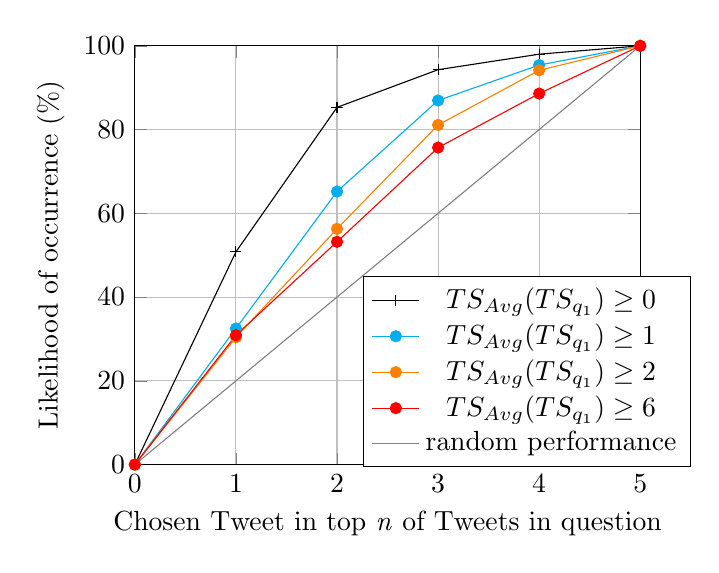
\begin{tikzpicture}
 \begin{axis}[
        xlabel=Chosen Tweet in top \textit{n} of Tweets in question,
        ylabel=Likelihood of occurrence (\%),
        grid = major,
        legend entries={$TS_{Avg}(TS_{q_1}) \geq 0 $, $ TS_{Avg}(TS_{q_1}) \geq 1 $, $TS_{Avg}(TS_{q_1}) \geq 2 $, $TS_{Avg}(TS_{q_1}) \geq 6 $, random performance},
        %legend style={nodes=right},
		%legend pos=south east,
		legend style={at={(1.1,0.45)}},
		%legend style={nodes=right, at={(0.6,0.5)},anchor=north},
		xmin=0, xmax=5,
		ymin=0, ymax=100	,
		width=8cm
		]
	\addplot[mark=+,black] plot coordinates {
        (0,0) (1,50.8) (2,85.3) (3,94.3) (4,98) (5,100)
        };
        
	\addplot[mark=*,cyan] plot coordinates {
        (0,0) (1,32.5) (2,65.2) (3,86.95) (4,95.4) (5,100)
        };
    \addplot[mark=*,orange] plot coordinates {
       (0,0) (1,30.4) (2,56.3) (3,81.1) (4,94.15) (5,100)
    };
    \addplot[mark=*,red] plot coordinates {
        (0,0) (1,30.9) (2,53.2) (3,75.7) (4,88.6) (5,100)
    };
    \addplot[gray] plot coordinates {
        (0,0) (1,20) (2,40) (3,60) (4,80) (5,100)
    };
\end{axis}
\end{tikzpicture}
}
\caption{The probability of the MTW's chosen Tweet's $TS_{Avg}(t)$ being in the top \textit{n} of Tweets for that question while varying the minimum allowed maximum Tweet score of the question.}
\label{fig:score-dist}
\end{figure}
Analyses were also conducted on the performance of the predictions on a per-question basis. Hereafter, a question, $q \in Q$, is defined as a set of Tweets where;
\[ q = {t^q_1, t^q_2, t^q_3, t^q_4, t^q_5} \]
and
\[ |q| = 5 \]

For conducting these question-based analyses, each question's five Tweets were ranked in order of ascending mean interestingness score such that $TS_{Avg}(t^q_1) \geq TS_{Avg}(t^q_2) \geq ... \geq TS_{Avg}(t^q_5)$. We then calculated the number of times the MTWs chose a Tweet that appeared in the top $n$ of the ranked list of Tweets, as shown in Figure \ref{fig:score-dist}.\\
In this figure, we vary the minimum allowed value of $TS_{Avg}(t^q_1)$ (the highest Tweet score in question $q$) to show how detecting more interesting Tweets was more accurate when the range of scores in each question is more disparate. We show, for cases in which $TS_{Avg}(q_1) \geq 1$, that the likelihood of the MTWs choosing one of our two most highly ranked Tweets of the question using the interestingness predictions is around 66\% and the chance that they choose one of the top three ranked Tweets is 87\%.

\subsubsection{Probability of Selection}

\begin{figure}[h]
\centering{
\begin{tikzpicture}
\pgfplotsset{every axis plot/.style={line width=2pt}}
 \begin{axis}[
        xlabel=$ x $,
        ylabel=$P(\text{t chosen} : TS_G(t) > x)$ ,
        grid = major,
        height=5.2cm, width=8cm,
        xmin=0, xmax=4
       ]
	\addplot+[smooth, mark=none]  table {5.Chapter3/data/cum-dist-score.dat};
\end{axis}
\end{tikzpicture}
}
\caption{The probability that Tweet $t$ is chosen given that $TS_G(t)$ is greater than a given value, $x$.}
\label{fig:score-cum-dist}
\end{figure}

Finally, we show that the probability of MTWs deciding a Tweet $t$ is interesting becomes higher as the value of $TS_G(t)$ increases. \\
In Figure \ref{fig:score-cum-dist}, although we exclude cases of Tweets with $TS_G(t) > 4$ to reduce noise (due to fewer samples), a significant increase in probability is observed, particularly in the interval 0-1 representing the range of Tweets that are uninteresting (fewer observed retweets than predicted) to `as expected' (observed retweet volume is equal to predicted). It is also illustrated that, from this initial work, Tweets with a predicted interestingness score of 3 or more are not significantly different from one another in terms of their `real', human-judged, interestingness. However, more work will be carried out towards this in the future so that more accurate research can be done on Tweets with scores of greater then 3 in this context.


\section{Further Analyses}
The interestingness scores have been validated in terms of there being recognition that they can signify interesting Tweets. This section will now continue onto some deeper analyses of the results in order to show \textit{how} it is able to work.

\subsection{Discerning Interesting Information from Noise}
In this subsection, the human-selected interestingness selection will be assessed. Of particular interest is the likelihood of humans agreeing on an interesting piece of information and the properties of the Tweet scores in questions when agreements \textit{are} made. \\
For this, analyses were made into the \textit{disparity} of scores for Tweets. That is, the range of scores of Tweets in a particular question and the effect this has on human decision in deducing interesting information.

\begin{table}[h]\footnotesize
\begin{center}
\begin{tabular}{ c | c | c | c }
	 Num. confident answers in $q$& min. $d^{Avg}(q)$ & max. $d^{Avg}(q)$ & avg. $d^{Avg}(q)$ \\
	 \hline
	0 & 0 & 846 & \textbf{17.6} \\
	> 0 & 0 & 1445 & 32.1 \\
	1 & 0 & 1445 & \textbf{34.3} \\
	> 1 & 0 & 4 & 0.647 \\
	> 2 & 0 & 0.55 & 0.204
\end{tabular}
\end{center}
\caption{Absolute $TS_{Avg}(t)$ disparity of questions with varying number of confident answers made. Entries in \textbf{bold} are used to highlight interesting values.}
\label{table:score_disparities}
\end{table}

The absolute Tweet score disparity for a question, $q$, is defined as $d(q)$. For example, for a disparity of average scores, this is calculated thus;

\[ d^{Avg}(q) = \max(TS_{Avg}(q)) - \min(TS_{Avg}(q)) \]

Table \ref{table:score_disparities} shows how the values for $TS(q)$ vary for questions with differing numbers of confident answers. A confident answer, as mentioned previously, is one where at least two MTWs have agreed on an interesting Tweet.\\
The data shows that the average $TS(q)$ is around double in cases where a question is answered with precisely one confident answers than in cases where there are no confident answers made. This indicates that a wider scale of interestingness in a question is useful for humans for picking out the content they'd prefer to read. If several pieces of content are more similarly interesting (or, as the case may be, uninteresting), then it becomes more difficult for an agreement to be made on which information is the \textit{most} interesting.\\
In addition, the average score disparities in cases where multiple confident answers were selected are very low. This helps to reinforce the notion that pieces of information that are very similar in terms of interest level make it hard for users to decide on the \textit{most} interesting. Indeed, in questions where this is the case, MTWs have selected, and agreed on, multiple Tweets.

 \begin{figure}[h]
\centering{
\begin{tikzpicture}
\pgfplotsset{every axis plot/.style={line width=2pt}}
 \begin{axis}[
        xlabel=Average $d^{Avg}(q)$,
        ylabel=Cumulative probability of a confident selection being made,
        grid = major,
        height=7.5cm, width=13cm,
       ]
	\addplot+[mark=none]  table {5.Chapter3/data/cum-question-disparity.dat};
\end{axis}
\end{tikzpicture}
}
\caption{The probability of a confident selection being made for question $q$ with varying $d(q)$.}
\label{fig:cum-question-disparity}
\end{figure}

To take this further, it is demonstrable that the probability of a confident selection being made for a particular question, $q$, increases as $TS(q)$ also increases (Figure \ref{fig:cum-question-disparity}.  Thus, this reinforces the notion that people find it easier to discern interesting information when compared to \textit{un}-interesting information. This, too, is highlighted in Table \ref{table:score_disparities_2}, in which it is shown that amongst \textit{all} questions (i.e. not only questions that have been confidently-answered) the score disparity is much smaller between Tweets that were selected than the score disparity for the entire question. \\
This is particularly the case in which there are a few Tweets which have similarly high scores amongst Tweets which collectively have \textit{lower} scores. Therefore, selecting confidently from the few Tweets with the similar scores become difficult, but it is demonstrated that these at least are \textit{more} interesting than the ones that weren't selected.\\

\begin{table}[h]\footnotesize
\begin{center}
\begin{tabular}{ l || c | c | c }
	   & $TS_G(t)$ &  $TS_U(t)$ &  $TS_{Avg}(t)$\\
	 \hline
	$TS_d(q)$ & 62.4 & 4.7 & 33.3\\
	$TS_{d_C}(q)$ & 35.3 & 3.1 & 19.0\\
	\hline
	Ratio & 57\% & 66\% & 58\%
\end{tabular}
\end{center}
\caption{Score disparity comparison between selected Tweets of question $q$ and \textit{all} Tweets in $q$ when using the three different Tweet scores as metrics}
\label{table:score_disparities_2}
\end{table}

For example, this data shows that, on average, the global score disparity for selected Tweets of a question, $q$, was only around 57\% that of the entire disparity of $q$.
